%File: anonymous-submission-latex-2025.tex
\documentclass[letterpaper]{article} % DO NOT CHANGE THIS
\usepackage[submission]{aaai25}  % DO NOT CHANGE THIS
\usepackage{times}  % DO NOT CHANGE THIS
\usepackage{helvet}  % DO NOT CHANGE THIS
\usepackage{courier}  % DO NOT CHANGE THIS
\usepackage[hyphens]{url}  % DO NOT CHANGE THIS
\usepackage{graphicx} % DO NOT CHANGE THIS
\urlstyle{rm} % DO NOT CHANGE THIS
\def\UrlFont{\rm}  % DO NOT CHANGE THIS
\usepackage{natbib}  % DO NOT CHANGE THIS AND DO NOT ADD ANY OPTIONS TO IT
\usepackage{caption} % DO NOT CHANGE THIS AND DO NOT ADD ANY OPTIONS TO IT
\usepackage{amsmath}
\frenchspacing  % DO NOT CHANGE THIS
\setlength{\pdfpagewidth}{8.5in} % DO NOT CHANGE THIS
\setlength{\pdfpageheight}{11in} % DO NOT CHANGE THIS
%
% These are recommended to typeset algorithms but not required. See the subsubsection on algorithms. Remove them if you don't have algorithms in your paper.
\usepackage{algorithm}
\usepackage{algorithmic}

%
% These are are recommended to typeset listings but not required. See the subsubsection on listing. Remove this block if you don't have listings in your paper.
\usepackage{newfloat}
\usepackage{listings}
\DeclareCaptionStyle{ruled}{labelfont=normalfont,labelsep=colon,strut=off} % DO NOT CHANGE THIS
\lstset{%
	basicstyle={\footnotesize\ttfamily},% footnotesize acceptable for monospace
	numbers=left,numberstyle=\footnotesize,xleftmargin=2em,% show line numbers, remove this entire line if you don't want the numbers.
	aboveskip=0pt,belowskip=0pt,%
	showstringspaces=false,tabsize=2,breaklines=true}
\floatstyle{ruled}
\newfloat{listing}{tb}{lst}{}
\floatname{listing}{Listing}
%
% Keep the \pdfinfo as shown here. There's no need
% for you to add the /Title and /Author tags.
\pdfinfo{
/TemplateVersion (2025.1)
}

% DISALLOWED PACKAGES
% \usepackage{authblk} -- This package is specifically forbidden
% \usepackage{balance} -- This package is specifically forbidden
% \usepackage{color (if used in text)
% \usepackage{CJK} -- This package is specifically forbidden
% \usepackage{float} -- This package is specifically forbidden
% \usepackage{flushend} -- This package is specifically forbidden
% \usepackage{fontenc} -- This package is specifically forbidden
% \usepackage{fullpage} -- This package is specifically forbidden
% \usepackage{geometry} -- This package is specifically forbidden
% \usepackage{grffile} -- This package is specifically forbidden
% \usepackage{hyperref} -- This package is specifically forbidden
% \usepackage{navigator} -- This package is specifically forbidden
% (or any other package that embeds links such as navigator or hyperref)
% \indentfirst} -- This package is specifically forbidden
% \layout} -- This package is specifically forbidden
% \multicol} -- This package is specifically forbidden
% \nameref} -- This package is specifically forbidden
% \usepackage{savetrees} -- This package is specifically forbidden
% \usepackage{setspace} -- This package is specifically forbidden
% \usepackage{stfloats} -- This package is specifically forbidden
% \usepackage{tabu} -- This package is specifically forbidden
% \usepackage{titlesec} -- This package is specifically forbidden
% \usepackage{tocbibind} -- This package is specifically forbidden
% \usepackage{ulem} -- This package is specifically forbidden
% \usepackage{wrapfig} -- This package is specifically forbidden
% DISALLOWED COMMANDS
% \nocopyright -- Your paper will not be published if you use this command
% \addtolength -- This command may not be used
% \balance -- This command may not be used
% \baselinestretch -- Your paper will not be published if you use this command
% \clearpage -- No page breaks of any kind may be used for the final version of your paper
% \columnsep -- This command may not be used
% \newpage -- No page breaks of any kind may be used for the final version of your paper
% \pagebreak -- No page breaks of any kind may be used for the final version of your paperr
% \pagestyle -- This command may not be used
% \tiny -- This is not an acceptable font size.
% \vspace{- -- No negative value may be used in proximity of a caption, figure, table, section, subsection, subsubsection, or reference
% \vskip{- -- No negative value may be used to alter spacing above or below a caption, figure, table, section, subsection, subsubsection, or reference

\setcounter{secnumdepth}{0} %May be changed to 1 or 2 if section numbers are desired.

% The file aaai25.sty is the style file for AAAI Press
% proceedings, working notes, and technical reports.
%

% Title

% Your title must be in mixed case, not sentence case.
% That means all verbs (including short verbs like be, is, using,and go),
% nouns, adverbs, adjectives should be capitalized, including both words in hyphenated terms, while
% articles, conjunctions, and prepositions are lower case unless they
% directly follow a colon or long dash
\title{Hidden Echoes Survive Training in Audio To Audio Generative Instrument Models}
\author{
    %Authors
    % All authors must be in the same font size and format.
    Christopher J. Tralie{\rm 1},\\
    Matt Amery,\\
    Benjamin Douglas,\\
    Ian Utz
}
\affiliations{
    %Afiliations
    \textsuperscript{\rm 1}Ursinus College Mathematics And Computer Science\\
    % If you have multiple authors and multiple affiliations
    % use superscripts in text and roman font to identify them.
    % For example,

    % Sunil Issar\textsuperscript{\rm 2},
    % J. Scott Penberthy\textsuperscript{\rm 3},
    % George Ferguson\textsuperscript{\rm 4},
    % Hans Guesgen\textsuperscript{\rm 5}
    % Note that the comma should be placed after the superscript
%
% See more examples next
}

%Example, Single Author, ->> remove \iffalse,\fi and place them surrounding AAAI title to use it
\iffalse
\title{My Publication Title --- Single Author}
\author {
    Author Name
}
\affiliations{
    Affiliation\\
    Affiliation Line 2\\
    name@example.com
}
\fi

\iffalse
%Example, Multiple Authors, ->> remove \iffalse,\fi and place them surrounding AAAI title to use it
\title{My Publication Title --- Multiple Authors}
\author {
    % Authors
    First Author Name\textsuperscript{\rm 1},
    Second Author Name\textsuperscript{\rm 2},
    Third Author Name\textsuperscript{\rm 1}
}
\affiliations {
    % Affiliations
    \textsuperscript{\rm 1}Affiliation 1\\
    \textsuperscript{\rm 2}Affiliation 2\\
    firstAuthor@affiliation1.com, secondAuthor@affilation2.com, thirdAuthor@affiliation1.com
}
\fi


% REMOVE THIS: bibentry
% This is only needed to show inline citations in the guidelines document. You should not need it and can safely delete it.
\usepackage{bibentry}
% END REMOVE bibentry

\begin{document}

\maketitle

\begin{abstract}

\end{abstract}

% Uncomment the following to link to your code, datasets, an extended version or similar.
%
% \begin{links}
%     \link{Code}{https://aaai.org/example/code}
%     \link{Datasets}{https://aaai.org/example/datasets}
%     \link{Extended version}{https://aaai.org/example/extended-version}
% \end{links}

\section{Preparing an Anonymous Submission}

\section{Introduction}

We use modified ideas from echo hiding \cite{gruhl1996echo}.

There are myriad techniques for generative audio instrument training (todo: citations), but to show the general applicability of this technique in a replicable way, we pick three open models with fundamentally different approaches whose code is readily available online: RAVE \cite{caillon2021rave} Dance Diffusion \cite{evans2022dancediffusion}, and differentiable digital signal processing (DDSP) \cite{engelddsp}.  Each model is trained on audio only, as opposed to those also involving language models (e.g. \cite{evans2024fast}) or MIDI (e.g. \cite{hawthornemulti}), and each model is trained on a collection of instrument sounds from the same instrument.  Specifically, we train models with different conditions on each of three open datasets to further enhance reproducibility: VocalSet \cite{wilkins2018vocalset}, Groove \cite{groove2019}, and GuitarSet \cite{xi2018guitarset}, which span vocals, and drums, and acoustic guitar, respectively.  We evaluate each model using the respective vocals, drums, and ``other'' stems in the MUSDB18-HQ dataset \cite{musdb18-hq} as inputs to models trained under various conditions.  This is a difficult audio watermarking scenario, as long moments of silence may be present in individual stems.




\section{Background}



\section{Methods}

Every audio sample in the training sets is converted to a 44100hz mono 

\subsection{Audio To Audio Models}

Explain RAVE and dance diffusion architectures

Specifics on architectures, with number of parameters

We use dance diffusion with a 81920 sample size, which means the receptive field spans about 1.86 seconds.  As the authors of \cite{hawthornemulti} note, using a network trained with a smaller context to synthesize audio clips may result in audible timbre shifts from one section to another; however, this is fine for a proof of concept.


\subsection{Echo Hiding}
\label{sec:echohiding}

\begin{figure}
    \centering
    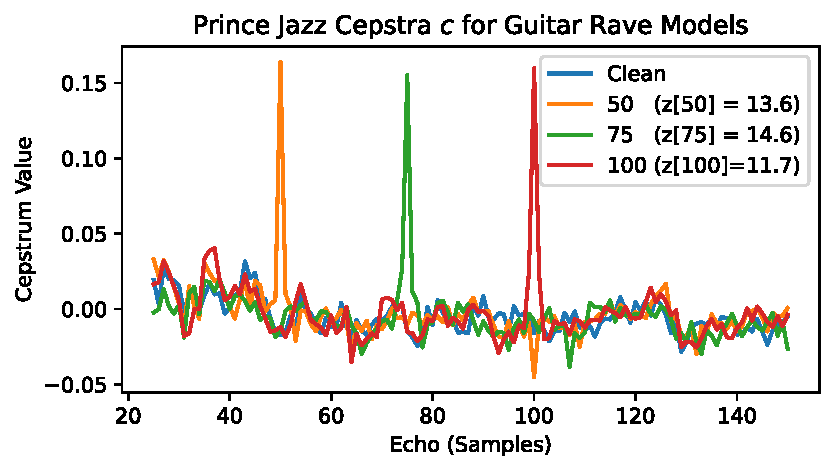
\includegraphics[width=\columnwidth]{figs/RaveCepstra.pdf}
    \caption{An example of cepstra computed on style transfer of a 30 second excerpt of a Prince jazz session at Loring Park.  Rave models trained on data with different echoes at 50, 75, and 100 lead to visible peaks at the respective places in their ceptra on the synthesized clips.}
    \label{fig:ravecepstra}
\end{figure}

Given a discrete audio ``carrier waveform'' $x$, audio watermarking techniques hide a binary payload in a watermarked waveform $\hat{x}$ so that $x$ and $\hat{x}$ are perceptually indistinguishable.  The original echo hiding paper by \cite{gruhl1996echo} accomplishes this by creating two waveforms $x_0$ and $x_1$, each with a single echo; 
\begin{equation}
    \begin{aligned}
        x_0[n] &= x[n] + \alpha x[n - \delta_0] \\
        x_1[n] &= x[n] + \alpha x[n - \delta_1]
    \end{aligned}
\end{equation}

 where $\alpha$ trades off perceptibility and robustness of the watermark and is generally much less than 1, and $\delta_0 = \delta_1$ are both less than 100 samples at a 44.1khz sample rate.  These waveforms are then mixed together in windows to create $\hat{x}$ according to the payload; where $x_0$ is fully mixed at the center of a window if the payload contains a 0 at that moment and $x_1$ is fully mixed in if the payload contains a 0.  For a window length of 1024 samples, for instance, this amounts to about 43 bits per second at 44.1khz.  Since convolution in the time domain is multiplication in the frequency domain, the logarithm of the magnitude of the DFT of a window additively separates the frequency response of the echo from the frequency response of the original signal.  Therefore, the so-called ``cepstrum'' of a windowed signal $x_w$:
 
\begin{equation}
    \label{eq:cepstrum}
    c = \text{ifft} ( \log ( | \text{fft} (x_w) | ) )
\end{equation}
 
yields a signal in which a single echo is a high peak, which is referred to as the ``cepstrum'' $c$ \footnote{\cite{gruhl1996echo} note that it is more mathematically correct take the {\em complex logarithm} of the DFT before taking the inverse DFT, and they further enhance with an autocorrelation.  But we found better results with the traditional cepstrum.}.  Thus, to decode the payload from the watermarked signal, one computes $c$ on each window and infers a 0 if $c[\delta_0] > c[\delta_1]$ or a 1 otherwise.

Since we seek to hide echoes in the training data for generative models, it is unlikely that the models we train will synthesize the windows in the same order they occur in the training set.  Therefore, we do away with the windowing completely and instead hide {\em the same echo} $\delta \in [50, 100]$ in {\em the entire audio clip} of {\em each waveform in the training data}.  We then examine the cepstrum $c$ of an entire clip that comes out of our models.  To score the cepstrum value at $\delta$ in a loudness-independent way, we compute the {\em z-score} at each lag $i$ as follows.  First, let $\mu_c[i]$ be the mean at $i$ excluding $i$:

\begin{equation}
    \mu_{c}[i] = \left( \sum_{j=25, 26, ..., i-1, i+1, 150} c[j] \right) / 125
\end{equation}

and let $\sigma_{c}[i]$ be 

\begin{equation}
    \sigma_{c}[i] = \sqrt{ \left( \sum_{j=25, 26, ..., i-1, i+1, 150} (c[j] - \mu_c[i])^2 \right) / 125}
\end{equation}

then

\begin{equation}
z[i]_{c} = \mu_{c}[i] / \sigma_{c}[i]
\end{equation}


A model trained on data watermarked with echo $\delta$ works well if $z[\delta] > z[i \neq \delta]$.  Figure~\ref{fig:ravecepstra} shows example cepstra from clips created with different Rave\cite{caillon2021rave} models trained on the GuitarSet \cite{xi2018guitarset} dataset, with various echoes $\delta$.  The peaks and z-scores show that the models reproduce the echoes they were trained on.  We will evaluate this more extensively in the experiment section (Figure~\ref{fig:singleechotable}).

\subsection{Pseudorandom Echo Patterns}

Though we have found single echoes to be robust, the information capacity is low.  Since we hide echoes between 50 and 100 at integer values, we can store at most ~5.6 bits of information in a single dataset.  To increase the information capacity, we also explore followup work on 





\section{Experiments}

\subsection{Single Echo Experiments}
\label{sec:experimentssingleecho}




\begin{figure}
    \centering
    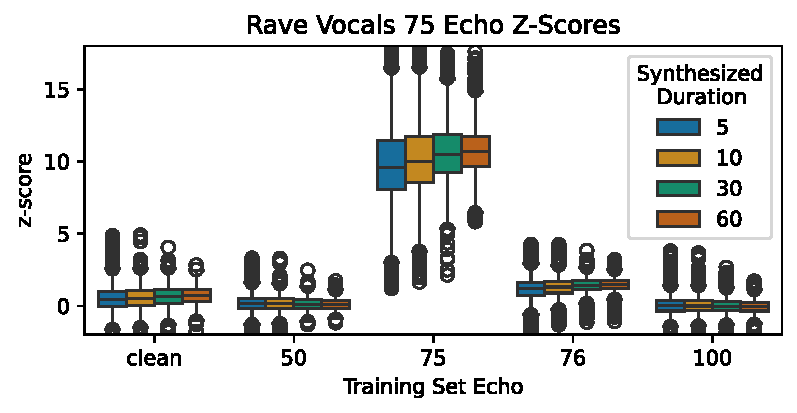
\includegraphics[width=\columnwidth]{figs/RaveZScoreExamples.pdf}
    \caption{As this example with various tagged vocalset training data shows, the z-scores for a 75 echo are much higher for the models that are trained on a dataset with a 75 echo embedded in every clip, and the separation increases with increasing clip duration.}
    \label{fig:ravezscoreexamples}
\end{figure}


\begin{figure}
    \centering
    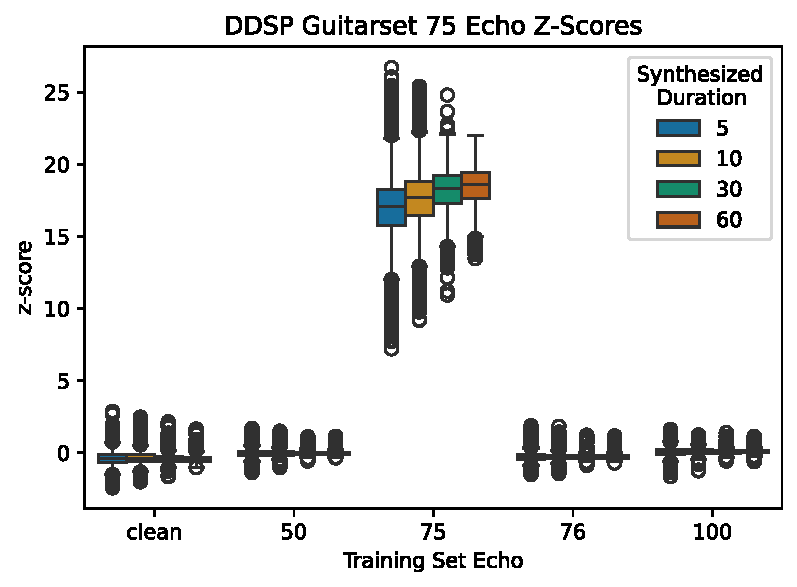
\includegraphics[width=\columnwidth]{figs/DDSPZScoreExamples.pdf}
    \caption{DDSP models show the strongest preservation of echoes, as measured by the z-score}
    \label{fig:ddspzscoreexamples}
\end{figure}

\begin{figure}
    \centering
    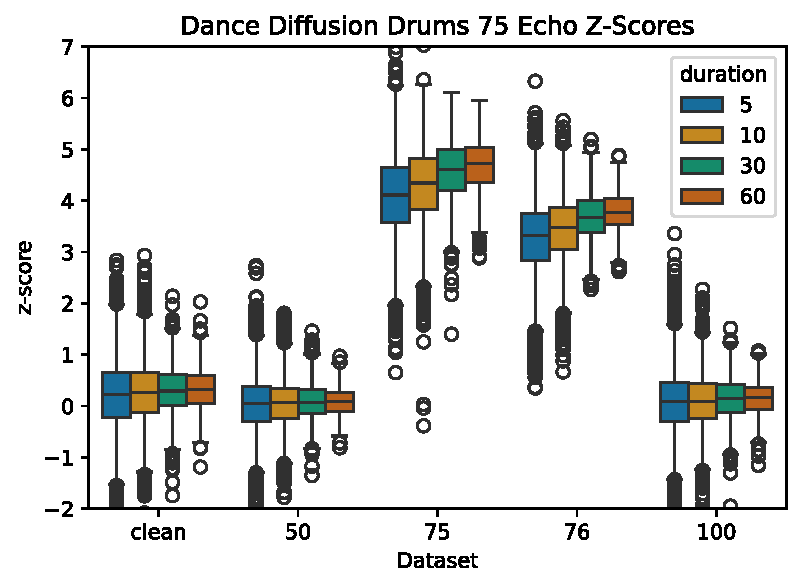
\includegraphics[width=\columnwidth]{figs/DanceDiffusionZScoreExamples.pdf}
    \caption{Dance diffusion models show slightly weaker z-scores that may be mixed up between adjacent echoes, but they still reproduce the correct echoes overall.}
    \label{fig:dancediffusionzscoreexamples}
\end{figure}


\begin{figure*}
    \centering
    \onecolumn
    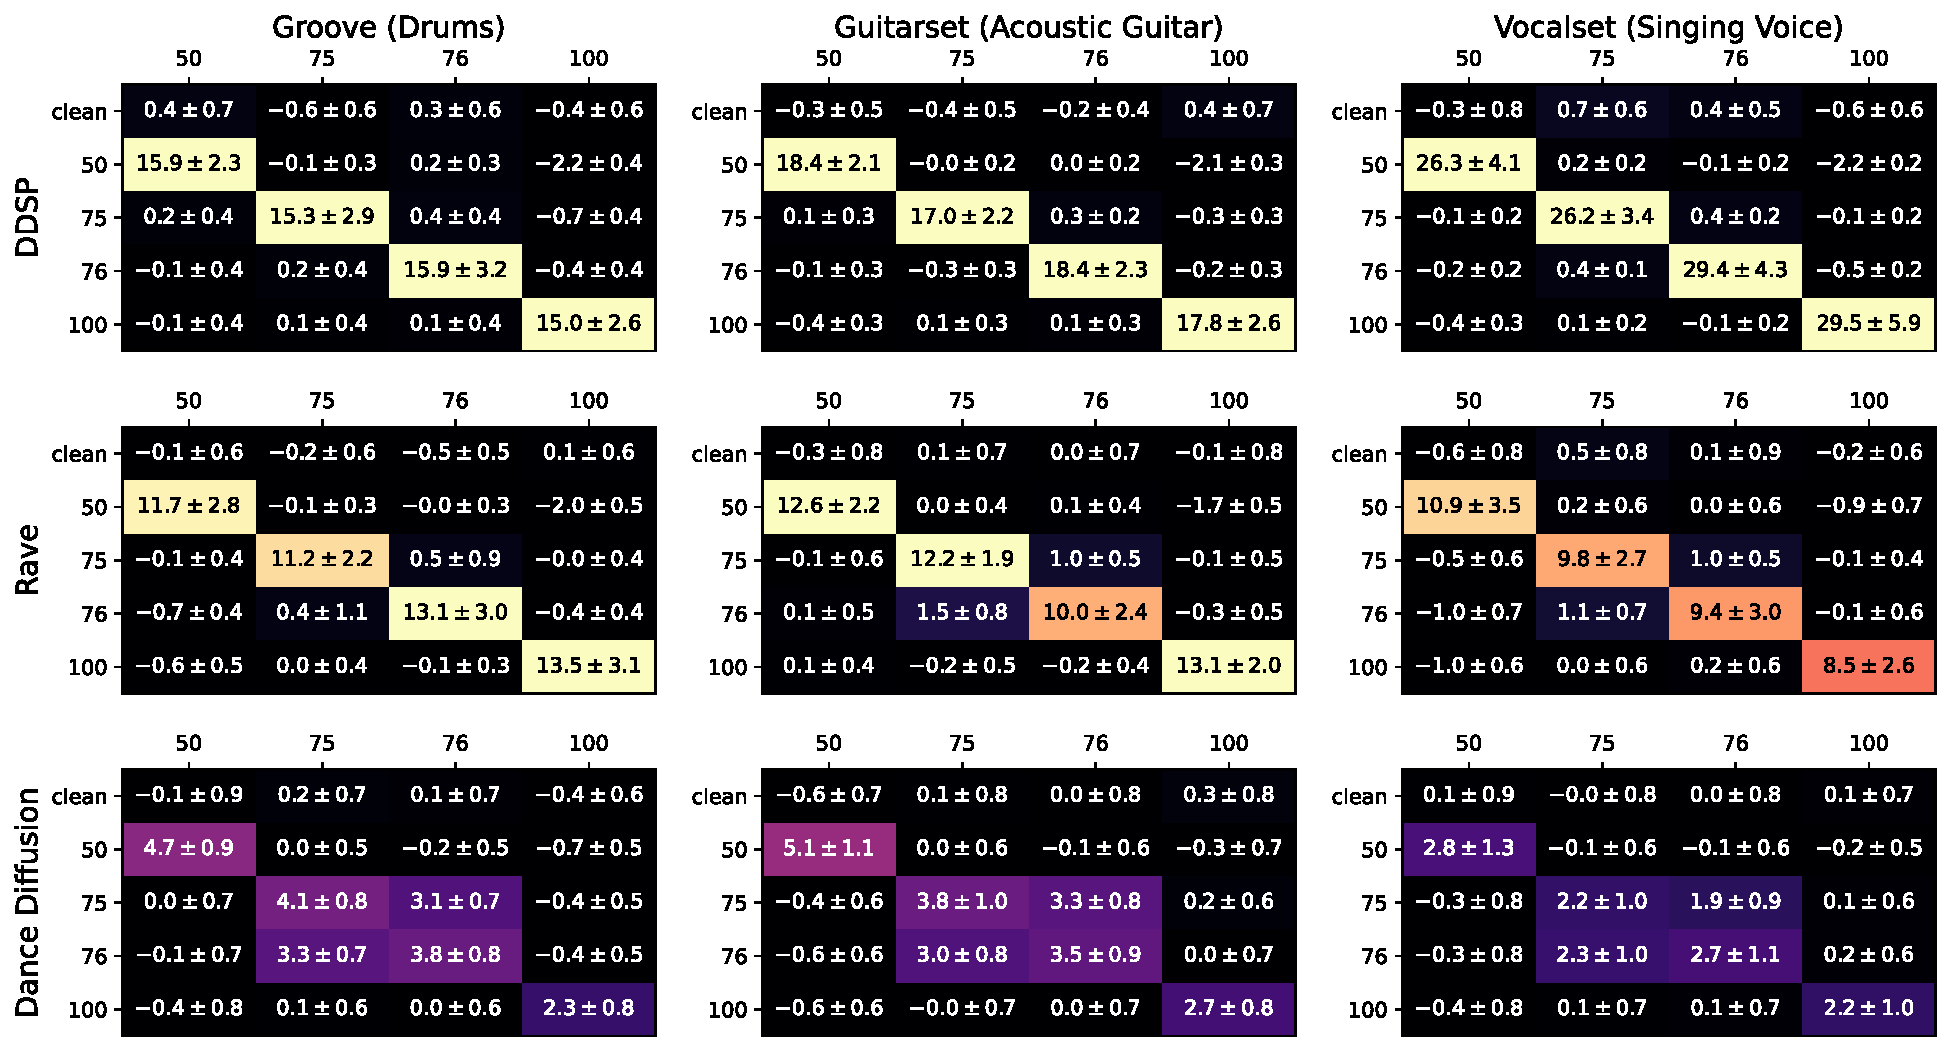
\includegraphics[width=\textwidth]{figs/AllSingleEchoZScores.pdf}
    
    \caption{Single echo results}
    \label{fig:singleechotable}
    \twocolumn
\end{figure*}


Explain musdb experiment

Table for 50, 75, 76, 100 for all instruments, plus percentage tagged for all models








\subsection{Pseudorandom Echo Sequences}

Time spread echo hiding \cite{ko2005time}.  We use kernels that are designed to be more robust \cite{xiang2010effective}, but we find they don't work as well

\section{Additional Use Cases}

We now explore thin slices through a few additional uses cases to highlight the versatility of the hidden echoes



\subsection{Dance Diffusion Fine Tuning}

Show results only on groove and vocalset since guitarset is too small


\subsection{Single Echo Demixing}



\subsection{Rave Pitch Shift Augmentation}



\subsection{Tagging Datasets}






\section{Conclusion}
The conclusion goes here.


\bibliography{writeup}

\end{document}
